\section{Einleitung}

Die Architektur besteht aus den folgenden zwei Haupt-Komponenten:
\begin{itemize}
	\item Eine Shared Codebase mit \emph{barefoot} \cite{Barefoot}
	\item Eine API-Komponente mit \emph{Express.js} \cite{Expressjs}
\end{itemize}

\begin{figure}[ht]
	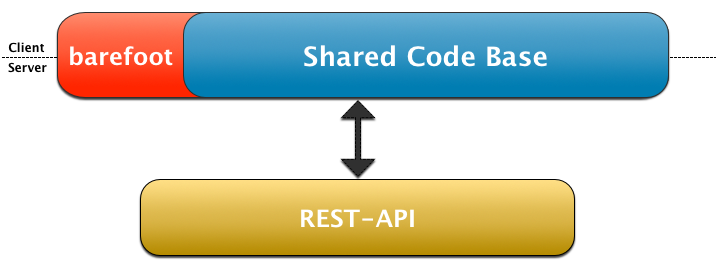
\includegraphics[width=\textwidth]{content/images/grob-layers-sad.png}
	\caption{Architektur}
\end{figure}

\subsection{Shared Codebase mit barefoot}
Barefoot \cite{Barefoot} ist ein Framework welches während der Bachelorarbeit entwickelt wurde.
Dieses Framework ermöglicht Client und Server den gleichen Code für Controller und Templates zu benutzen und setzt auf
Backbone.js \cite{Backbonejs} für die Code-Strukturierung auf.

Als Beispiel sei hier der Router genannt:
\begin{lstlisting}[language=JavaScript, caption=Router der Beispielapplikation \cite{roomiesRouter}, label=lst:roomiesRouter, firstnumber=25]
module.exports = Router.extend({
	routes: {
		'': 'home'
		, 'community': 'createCommunity'
		//...
	}

	/** Function: home
	 * Home page which renders the login button if not authorized.
	 * Otherwise it redirects to community/create or community/:slug/tasks.
	 */
	, home: function home() {
		if(!this.isAuthorized()) {
			this.render(this.createView(HomeView));
		} else {
			var community = this.dataStore.get('community');
			if(!community) {
				this.navigate('community/create', { trigger: true });
			} else {
				this.navigate('community/' + community.get('slug') +
					'/tasks', { trigger: true });
			}
		}
	}

	/** Function: createCommunity
	 * Create community view
	 */
	, createCommunity: function createCommunity() {
		debug('create community');
		if(!this.redirectIfNotAuthorized()) {
			this.render(this.createView(CreateCommunityView));
		}
	}
	//...
});
\end{lstlisting}

Quelltext \ref{lst:roomiesRouter} zeigt ein Auszug des Routers aus der Beispielapplikation.
Dieser Router wird sowohl vom Client wie auch vom Server direkt verwendet und registriert die gezeigten URLs mit den Funktionen.

Wie man sieht, wird für die ``home''-Route, falls der Besucher nicht eingeloggt ist,
die ``HomeView'' dargestellt. Diese ist im Quellcode \ref{lst:roomiesHomeView}, ``\nameref{lst:roomiesHomeView}'' zu sehen.

\begin{lstlisting}[language=JavaScript, caption=HomeView der Beispielapplikation \cite{roomiesHomeView}, label=lst:roomiesHomeView, firstnumber=7]
module.exports = View.extend({
	el: '#main'
	, template: templates.login

	/** Function: renderView
	 * Renders the home view.
	 */
	, renderView: function renderView() {
		this.$el.html(this.template({}));
	}

	/** Function: afterRender
	 * Sets the document title.
	 */
	, afterRender: function afterRender(resolve) {
		var _super = this.constructor.__super__.afterRender.bind(this);

		this.setDocumentTitle(this.translate('Welcome'));
		_super(resolve);
	}
	//...
});
\end{lstlisting}

\subsection{API-Komponente}
Damit sichergestellt werden kann, dass alle Daten valid sind, ist auf Server-Seite
eine REST-API \cite{REST} erstellt worden. Die Shared Codebase greift auf diese zu, um
Daten zu speichern oder zu laden.
Dabei unterscheidet ``barefoot'' intelligent zwischen API-Aufrufen vom Server oder vom Client.
Wird vom Client aus aufgerufen, wird ein normaler AJAX-Aufruf gemacht. Wird die API
hingegen vom Server aus aufgerufen, werden direkt die entsprechend definierten
Callbacks für die gewünschte Route aufgerufen.

Der Quellcode \ref{lst:roomiesControllerExample} zeigt ein Beispiel für einen solchen
Callback, während Quelltext \ref{lst:roomiesComponentExample} ein Beispiel für
eine definierte API-Route aufzeigt.

\begin{lstlisting}[language=JavaScript, caption=API-Controller Beispiel \cite{roomiesCommunityApiExample}, label=lst:roomiesControllerExample, firstnumber=294]
/** Function: getCommunityWithId
 * Looks up a community with a specific ID.
 *
 * Parameters:
 *   (Function) success - Callback on success. Will pass the community data
 *                        as first argument.
 *   (Function) error - Callback in case of an error
 *   (String) id - The id of the community to look for.
 */
function getCommunityWithId(success, error, id) {
	debug('get community with id');

	var communityDao = getCommunityDao.call(this)

		/* AnonymousFunction: forwardError
		 * Forwards an error object using the error callback argument
		 */
		, forwardError = function forwardError(err) {
			return error(err);
		}

		/* AnonymousFunction: afterCommunitySearch
		 * Calls the success or error callback after searching for a community.
		 */
		, afterCommunitySearch = function afterCommunitySearch(community) {
			if(!_.isNull(community)) {
				success(community.dataValues);
			} else {
				forwardError(new errors.NotFoundError(
					'Community with id ' + id + 'does not exist.')
				);
			}
		};

	communityDao.find({ where: { id: id, enabled: true }})
		.success(afterCommunitySearch)
		.error(forwardError);
}
\end{lstlisting}

\begin{lstlisting}[language=JavaScript, caption=API-Route Beispiel \cite{communityApiDefinition}, label=lst:roomiesComponentExample, firstnumber=31]
var prefix = apiPrefix + modulePrefix;

// GET /api/community/:id
api.get(prefix + '/:id(\\d+)', [
	basicAuthentication
	, authorizedForCommunity
	, controller.getCommunityWithId]);
\end{lstlisting}

Die Beispielapplikation ist somit nach einem MVC-Pattern aufgebaut. \\
Die einzelnen Komponenten haben folgende Aufgabe:
\begin{itemize}
	\item{\textbf{M}odel ist das traditionelle Model welches zwischen Server \& Client geshared wird}
	\item{\textbf{V}iew ist eine ``Barefoot.View'' \cite{BarefootView} und rendert Templates}
	\item{\textbf{C}ontroller ist einerseits ein ``Route''-Controller, welcher aufgrund von URLs die richtige View aufruft und andererseits ein API-Controller, welcher die REST-API-Logik kapselt}
\end{itemize}

Diagramm \ref{fig:mvcComponentDiagramm} zeigt eine grobe Übersicht über das Zusammenspiel der verschiedenen Komponenten.

\begin{figure}[ht!]
	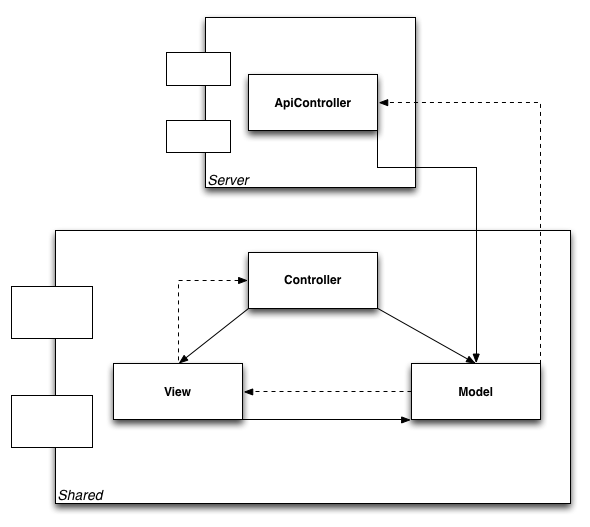
\includegraphics[width=\textwidth]{content/images/mvc-components.png}

	\caption{MVC-Komponenten im Zusammenspiel}
	\label{fig:mvcComponentDiagramm}
\end{figure}